\chapter{UJI COBA DAN EVALUASI}

Pada bab ini dijelaskan tentang uji coba dan evaluasi dari implementasi yang telah dilakukan pada Tugas Akhir ini.

\section{Lingkungan Uji Coba}

Linkungan uji coba yang digunakan adalah salah satu sistem yang digunakan situs penilaian daring SPOJ, yaitu kluster \textit{Cube} dengan spesifikasi sebagai berikut:

\begin{enumerate}
	\item Perangkat Keras:
	\begin{itemize}
		\item \textit{Processor} Intel(R) Pentium G860 CPU @ 3GHz.
		\item \textit{Memory} 1536 MB.
	\end{itemize}
	\item Perangkat Lunak:
	\begin{itemize}
		\item \textit{Compiler} g++ versi 4.3.2.
	\end{itemize}			
\end{enumerate} 

\section{Uji Coba Kebenaran}
\label{section:ujikebenaran}
Uji coba kebenaran dilakukan dengan analisis penyelesaian sebuah contoh kasus menggunakan pendekatan penyelesaian yang telah dijelaskan pada subbab \ref{chapter:rope} serta pengumpulan berkas kode sumber hasil implementasi ke dalam situs penilaian daring SPOJ.\\
Kasus yang akan digunakan sebagai bahan uji kebenaran dalam analisis penyelesaian \problem{} menggunakan contoh kasus pada Gambar \ref{figure:sample_problem}.
\begin{figure}[h]
	%\inputminted[frame=lines]{text}{bab5/rope.in} %
	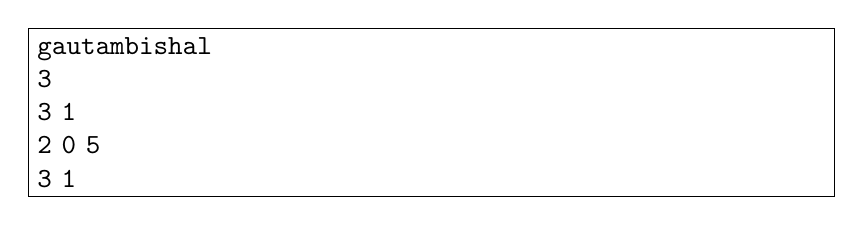
\begin{tikzpicture}
	\node (example-align) [draw, text width=10cm, align=left, font=\ttfamily]{gautambishal \\3\\3 1\\2 0 5\\3 1};
	\end{tikzpicture}
	\caption{Contoh kasus uji permasalahan Alphabetic Rope}
	\label{figure:sample_problem}
\end{figure}\\
Mula-mula dalam setiap permasalahan adalah membangun struktur \textit{rope} yang sesuai dengan \textit{string} masukan. Operasi dasar pada sebuah \textit{rope} adalah fungsi Insert, dimana dibentuk sebuah \textit{tree} yang berfungsi untuk menyimpan potongan karakter pada \textit{rope}. Selanjutnya \textit{rope} akan dibangun pada \textit{node root} yang dilakukan berdasarkan posisi tengah dari panjang \textit{string}. Pembentukan ini dapat dilihat pada Gambar \ref{fig:build_root}. Nilai pada tanda kurung siku menyatakan isi karakter pada \textit{node} tersebut. Dikarenakan masih terdapat \textit{string} yang tersisa maka proses pembentukan dilanjutkan untuk membentuk anak kiri dan anak kanan \textit{root}.
\begin{figure}[h]
\centering
\begin{tikzpicture}[->,>=stealth', level/.style={sibling distance = 5cm/#1, level distance = 1.5cm}, scale=0.93,transform shape]
\node {
	[b]
	\begin{tabular}{|c|c|c|c|c|c|c|c|c|c|c|c|}
		\hline
		g & a & u & t & a & m & b & i & s & h & a & l\\ \hline
		\nc{0} & \nc{1} & \nc{2} & \nc{3} & \nc{4} & \nc{5} & \nc{6} & \nc{7} & \nc{8} & \nc{9} & \nc{10} & \nc{11}\\
	\end{tabular}
};
\end{tikzpicture}
\caption{Pembentukan \textit{Root Rope} \label{fig:build_root}}
\end{figure}
Rentang \textit{string} pada anak kiri diperoleh dari indeks $0$ hingga nilai tengah$-1$ sedangkan rentang kanan diperoleh dari nilai tengah$+1$ hingga panjang \textit{string}. Pembentukan anak dari \textit{root} ditunjukkan pada Gambar \ref{fig:build_level1}. Pada setiap anak kiri dan anak kanan, posisi karakter yang berada ditengah-tengah \textit{string} anak menjadi nilai dari \textit{node} tersebut. Yang ditunjukkan oleh nilai di dalam tanda kurung siku.
\begin{figure}[h]
\centering
\begin{tikzpicture}[->,>=stealth', level/.style={sibling distance = 5cm/#1, level distance = 1.5cm}, scale=0.93,transform shape]
\node {
	[b]
	\begin{tabular}{|c|c|c|c|c|c|c|c|c|c|c|c|}
		\hline
		g & a & u & t & a & m & b & i & s & h & a & l\\ \hline
		\nc{0} & \nc{1} & \nc{2} & \nc{3} & \nc{4} & \nc{5} & \nc{6} & \nc{7} & \nc{8} & \nc{9} & \nc{10} & \nc{11}\\
	\end{tabular}
}
child {
	node {
		[t]
		\begin{tabular}{|c|c|c|c|c|c|}
			\hline
			g & a & u & t & a & m\\ \hline
			\nc{0} & \nc{1} & \nc{2} & \nc{3} & \nc{4} & \nc{5}\\
		\end{tabular}
	}
} 
child {
	node {
		[h]
		\begin{tabular}{|c|c|c|c|c|}
			\hline
			i & s & h & a & l\\ \hline
			\nc{7} & \nc{8} & \nc{9} & \nc{10} & \nc{11}\\
		\end{tabular}
	}
};
\end{tikzpicture}
\caption{Pembentukan \textit{Rope} pada Tingkat ke-$2$ \label{fig:build_level1}}
\end{figure}\\
Dikarenakan masih terdapat \textit{string} yang tersisa, proses pembentukan dilanjutkan untuk tingkat ke-$3$ yang ditunjukkan pada Gambar \ref{fig:build_level2}.
\begin{figure}[h]
\centering
\begin{tikzpicture}[->,>=stealth', level/.style={sibling distance = 8cm/#1, level distance = 1.5cm}, scale=0.7,transform shape]
\node {
	[b]
	\begin{tabular}{|c|c|c|c|c|c|c|c|c|c|c|c|}
		\hline
		g & a & u & t & a & m & b & i & s & h & a & l\\ \hline
		\nc{0} & \nc{1} & \nc{2} & \nc{3} & \nc{4} & \nc{5} & \nc{6} & \nc{7} & \nc{8} & \nc{9} & \nc{10} & \nc{11}\\
	\end{tabular}
}
child {
	node {
		[t]
		\begin{tabular}{|c|c|c|c|c|c|}
			\hline
			g & a & u & t & a & m\\ \hline
			\nc{0} & \nc{1} & \nc{2} & \nc{3} & \nc{4} & \nc{5}\\
		\end{tabular}
	}
	child {
		node{
			[a]
			\begin{tabular}{|c|c|c|}
				\hline
				g & a & u\\ \hline
				\nc{0} & \nc{1} & \nc{2}\\
			\end{tabular}
		}
	}
	child {
		node{
			[m]
			\begin{tabular}{|c|c|}		
				\hline
				a & m\\ \hline
				\nc{4} & \nc{5}\\
			\end{tabular}
		}
	}
} 
child {
	node {
		[h]
		\begin{tabular}{|c|c|c|c|c|}
			\hline
			i & s & h & a & l\\ \hline
			\nc{7} & \nc{8} & \nc{9} & \nc{10} & \nc{11}\\
		\end{tabular}
	}
	child {
		node{
			[s]
			\begin{tabular}{|c|c|}		
				\hline
				i & s\\ \hline
				\nc{7} & \nc{8}\\
			\end{tabular}
		}
	}
	child {
		node{
			[l]
			\begin{tabular}{|c|c|}		
				\hline
				a & l\\ \hline
				\nc{10} & \nc{11}\\
			\end{tabular}
		}
	}
};
\end{tikzpicture}
\caption{Pembentukan \textit{Rope} pada Tingkat ke-$3$ \label{fig:build_level2}}
\end{figure}\\
Untuk tahap selanjutnya dilakukan pembentukan \textit{rope} pada tingkat ke-$4$ yang ditunjukkan pada Gambar \ref{fig:arope}.
\begin{figure}[h]
\centering
\begin{tikzpicture}[->,>=stealth', level/.style={sibling distance = 8cm/#1, level distance = 1.5cm}, scale=0.68,transform shape]
\node {
	[b]
	\begin{tabular}{|c|c|c|c|c|c|c|c|c|c|c|c|}
		\hline
		g & a & u & t & a & m & b & i & s & h & a & l\\ \hline
		\nc{0} & \nc{1} & \nc{2} & \nc{3} & \nc{4} & \nc{5} & \nc{6} & \nc{7} & \nc{8} & \nc{9} & \nc{10} & \nc{11}\\
	\end{tabular}
}
child {
	node {
		[t]
		\begin{tabular}{|c|c|c|c|c|c|}
			\hline
			g & a & u & t & a & m\\ \hline
			\nc{0} & \nc{1} & \nc{2} & \nc{3} & \nc{4} & \nc{5}\\
		\end{tabular}
	}
	child {
		node{
			[a]
			\begin{tabular}{|c|c|c|}
				\hline
				g & a & u\\ \hline
				\nc{0} & \nc{1} & \nc{2}\\
			\end{tabular}
		}
		child {
			node {
				[g]
				\begin{tabular}{|c|}
					\hline
					g\\ \hline
				\end{tabular}
			}
		}
		child {
			node {
				[u]
				\begin{tabular}{|c|}
					\hline
					u\\ \hline
				\end{tabular}
			}
		}
	}
	child {
		node{
			[m]
			\begin{tabular}{|c|c|}		
				\hline
				a & m\\ \hline
				\nc{4} & \nc{5}\\
			\end{tabular}
		}
		child {
			node {
				[a]
				\begin{tabular}{|c|}
					\hline
					a\\ \hline
				\end{tabular}
			}
		}
		child[missing]{}
	}
} 
child {
	node {
		[h]
		\begin{tabular}{|c|c|c|c|c|}
			\hline
			i & s & h & a & l\\ \hline
			\nc{7} & \nc{8} & \nc{9} & \nc{10} & \nc{11}\\
		\end{tabular}
	}
	child {
		node{
			[s]
			\begin{tabular}{|c|c|}		
				\hline
				i & s\\ \hline
				\nc{7} & \nc{8}\\
			\end{tabular}
		}
		child {
			node {
				[i]
				\begin{tabular}{|c|}
					\hline
					i\\ \hline
				\end{tabular}
			}
		}
		child[missing]{}
	}
	child {
		node{
			[l]
			\begin{tabular}{|c|c|}		
				\hline
				a & l\\ \hline
				\nc{10} & \nc{11}\\
			\end{tabular}
		}
		child {
			node {
				[a]
				\begin{tabular}{|c|}
					\hline
					a\\ \hline
				\end{tabular}
			}
		}
		child[missing]{}
	}
};
\end{tikzpicture}
\begin{tikzpicture}[level/.style={sibling distance = 8cm/#1, level distance = 1.5cm}, scale=0.68,transform shape]
\node[treenode]{b,12}
  child{
    node[treenode]{t,6} 
    child {
    	node[treenode] {a,3}
    	child {
    		node[treenode]{g,1}
    	}
    	child{
    		node[treenode] {u,1}
    	}
    }
    child {
    	node[treenode] {m,2}
    	child {
    	    node[treenode] {a,1}
    	}
    	child[missing]{}
    }
  }
  child{
  	node[treenode]{h,5}
  	child {
  	    	node[treenode] {s,2}
  	    	child {
  	    		node[treenode]{i,1}
  	    	}
  	    	child[missing]{}
  	    }
  	    child {
  	    	node[treenode] {l,2}
  	    	child {
  	    	    node[treenode] {a,1}
  	    	}
  	    	child[missing] {}
  	    }
  };
\end{tikzpicture}
\caption{Struktur \textit{Rope} yang Terbentuk \label{fig:arope}}
\end{figure}\\
\textit{Query} pertama memiliki parameter $type \gets 3$, $y \gets 0$. Tahapan pertama dengan mencari karakter pada indeks ke-$y$. Untuk memperoleh jawaban dilakukan penelusuran sesuai dengan algoritma yang dijelaskan pada subbab \ref{chapter:index}.

Tahapan pencarian pada \textit{rope} adalah sebagai berikut,

$y \gets 1$, $left.weight \gets 6$, $idx \gets left.weight$; $idx <= y$;
dilanjutkan ke anak kiri;

$y \gets 1$, $left.weight \gets 3$, $idx \gets left.weight$; $idx <= y$;
dilanjutkan ke anak kiri;

$y \gets 1$, $left.weight \gets 1$, $idx \gets left.weight$; $idx \gets y$;
kembalikan nilai \textit{node} saat ini;

Maka jawaban untuk \textit{query} ini adalah $a$. 

\textit{Query} kedua memiliki parameter $type \gets 2$, $x \gets 0$, $y \gets 5$. Proses perubahan pada \textit{rope} adalah sebagai berikut,

$x \gets 0$, $y \gets 5$, $left.weight \gets 6$, $idx \gets left.weight$; $idx <= y$;
dilanjutkan ke anak kiri;

$x \gets 0$, $y \gets 5$, $left.weight \gets 3$, $idx \gets left.weight$; $idx <= y$;
dilanjutkan ke anak kiri;

$x \gets 0$, $y \gets 5$, $left.weight \gets 1$, $idx \gets left.weight$; $idx <= y$;
dilanjutkan ke anak kiri;

$x \gets 0$, $y \gets 5$, $left.weight \gets 0$, $idx \gets left.weight$; $idx \gets y$;
kembalikan nilai \textit{node} saat ini;

Dikarenakan $x \gets 0$ operasi Split menghasilkan \textit{rope} $R_1$ yang berisi NULL dan $R_2$ sisa dari potongan \textit{rope} yang berarti keseluruhan \textit{rope} saat ini.

Proses perubahan selanjutnya adalah sebagai berikut,

$x \gets 0$, $y \gets 5$, $left.weight \gets 1$, $len \gets y - x + 1$, $idx \gets left.weight$; $idx = len$;
kembalikan nilai \textit{node} saat ini;

Setelah menemukan posisi \textit{node} yang akan dipotong, hapus sambungan dari seluruh \textit{node} yang memiliki nilai indeks kurang dari nilai indeks saat ini. Hasil potongan dari \textit{rope} akan disimpan dengan menggunakan struktur data Pair yang bertipe \textit{pointer node}. Sehingga menghasilkan dua buah \textit{rope} baru $R_{21}$ yang berisi \textit{string} "$gautam$" dan $R_{22}$ yang berisi \textit{string} "$bishal$".

Potongan \textit{rope} yang baru terbentuk akan digabungkan berdasarkan $type \gets 2$, dimana $R_{21}$ berada diposisi belakang dari keseluruhan \textit{rope}. Konfigurasi \textit{rope} yang baru terbentuk berisi \textit{string} "$bishalgautam$" yang ditunjukkan pada Gambar \ref{fig:konfigurasi-3}.
\begin{figure}[h]
\centering
\begin{tikzpicture}[level/.style={sibling distance = 5cm/#1, level distance = 1.5cm},  scale=0.7,transform shape]
\node[treenode]{t,12}
child {
	node[treenode]{a,9}
	child {
		node[treenode]{b,7}
		child[missing]{}
		child {
			node[treenode]{h,6}
			child {
				node[treenode]{s,2}
				child {
					node[treenode]{i,1}
				}
				child[missing]{}
			}
			child {
				node[treenode]{g,3}
				child {
					node[treenode]{l,2}
					child {
						node[treenode]{a,1}
					}
					child[missing]{}
				}
				child[missing]{}
			}
		}
	}
	child {
		node[treenode]{u,1}
	}
}
child {
	node[treenode]{m,2}
	child {
		node[treenode]{a,1}
	}
	child[missing]{}
};
\end{tikzpicture}
\caption{Konfigurasi \textit{Rope} Setelah Operasi $2$ $0$ $5$ \label{fig:konfigurasi-3}}
\end{figure}

\textit{Query} ketiga memiliki parameter $type \gets 3$, $y \gets 0$. Proses perubahan dan pencarian pada \textit{rope} adalah sebagai berikut,

$y \gets 0$, $left.weight \gets 9$, $idx \gets left.weight$; $idx <= y$;
dilanjutkan ke anak kiri;

$y \gets 0$, $left.weight \gets 7$, $idx \gets left.weight$; $idx <= y$;
dilanjutkan ke anak kiri;

$y \gets 0$, $left.weight \gets 0$, $idx \gets left.weight$; $idx \gets y$;
kembalikan nilai \textit{node} saat ini;

Maka jawaban untuk \textit{query} ini adalah $b$.

Secara terurut jawaban dari kedua \textit{query} tersebut adalah $a$ dan $b$. Kemudian sistem penyelesaian dijalankan dan diberi masukan sesuai kasus uji dari analisis sebelumnya dan hasil luaran sistem adalah $a$ dan $b$ seperti terlihat pada Gambar \ref{fig:hasil-luaran}.
\begin{figure}[H]
\centerline{ \includegraphics[scale=0.6]{assets/images/hasil.png}}
\caption{Hasil Luaran Program pada Contoh Kasus Uji Alphabetic Rope}
\label{fig:hasil-luaran}
\end{figure}

Selanjutnya dilakukan juga uji coba kebenaran dengan mengirimkan kode sumber program ke dalam situs penilaian daring SPOJ. Permasalahan yang diselesaikan adalah \problem{}. Hasil uji kebenaran dan waktu eksekusi program pada saat pengumpulan kasus uji pada situs SPOJ ditunjukkan pada Gambar \ref{figure:ujicoba}.
\begin{figure}[H]
\centerline{ \includegraphics[scale=0.43]{assets/images/ujicoba.png}}
\caption{Hasil Uji Coba pada Situs Penilaian SPOJ}
\label{figure:ujicoba}
\end{figure}

Hal ini membuktikan bahwa implementasi yang dilakukan telah berhasil menyelesaikan \problem{} dengan batasan-batasan yang telah ditetapkan. Setelah itu dilakukan pengiriman kode sumber implementasi sebanyak 15 kali untuk melihat variasi waktu dan memori yang dibutuhkan program. Hasil uji coba sebanyak $15$ kali dapat dilihat pada Gambar \ref{figure:submission}. Grafik hasil uji coba sebanyak 15 kali ditunjukkan pada Gambar \ref{figure:grafik_spam}.
\begin{figure}[H]
\centerline{ \includegraphics[scale=0.5]{assets/images/spoj-spam.png}}
\caption{Hasil Uji Coba pada Situs Penilaian SPOJ}
\label{figure:grafik_spam}
\end{figure}
\begin{table}{}
	\centering
	\begin{tabular}{|c|c|}
	\hline
		Waktu Maksimal & $0.16$ detik\\ \hline
		Waktu Minimal & $0.14$ detik\\ \hline
		Waktu Rata-Rata & $0.152$ detik\\ \hline
		Memori Maksimal & $5.0$ MB\\ \hline
		Memori Minimal & $5.0$ MB\\ \hline
		Memori Rata-rata & $5.0$ MB\\ \hline
	\end{tabular}\caption{Kecepatan Maksimal, Minimal dan Rata-Rata dari Hasil Uji Coba Sebanyak 15 Kali pada Situs Pengujian SPOJ \label{tab:pengujian}}
\end{table}
Berdasarkan Tabel \ref{tab:pengujian} dari percobaan pengujian yang dilakukan, didapat waktu rata-rata program yaitu $0.152$ detik dan penggunaan memori yang dibutuhkan program yaitu $5.0$ MB. Hasil ini masih dibawah dari batas maksimal waktu dan memori pada \problem{}, yaitu $1$ detik dan $1536$ MB.

\section{Uji Coba Kinerja}
\label{section:ujikinerja}
Uji coba kinerja penyelesaian \problem{} dilakukan dengan cara membandingkan waktu yang dibutuhkan untuk penyelesaian menggunakan \textit{string} dengan struktur data Rope yang dibuat.
\subsection{Operasi 1 Menggabungkan \textit{Rope} pada Posisi Awal}
Pada Gambar \ref{figure:operasi1string} terlihat bahwa untuk $N \gets 5000$ sampai $N \gets 10^5$ dengan banyak $Q \gets 10^5$, struktur Rope yang dibuat untuk penyelesaian \problem{} menunjukkan waktu yang lebih cepat dibandingan dengan algoritma String dan stuktur data Rope pembanding. Sedangkan untuk $N \gets 10^5$ dengan $Q \gets 5000$ sampai $Q \gets 10^5$, pertumbuhan waktu secara logaritmik dan lebih kecil dibandingkan dengan algoritma String dan struktur data Rope pembanding yang ditunjukkan pada Gambar \ref{figure:operasi1query}. Untuk tabel performa antara algoritma String dengan struktur data Rope yang telah dibuat dapat dilihat pada Tabel \ref{tab:operasi1string} dan \ref{tab:operasi1query}.
\begin{figure}
\centerline{ \includegraphics[scale=0.45]{assets/images/operasi1-string.png}}
\caption{Hasil Uji Coba pada Operasi 1 dengan Jumlah \textit{Query} Tetap dan Panjang \textit{String} Bertambah}
\label{figure:operasi1string}
\end{figure}

\begin{figure}
\centerline{ \includegraphics[scale=0.45]{assets/images/operasi1-query.png}}
\caption{Hasil Uji Coba pada Operasi 1 dengan Jumlah \textit{String} Tetap dan Jumlah \textit{Query} Bertambah}
\label{figure:operasi1query}
\end{figure}

\subsection{Operasi 2 Menggabungkan \textit{Rope} pada Posisi Akhir}
Pada Gambar \ref{figure:operasi2string} terlihat bahwa untuk $N \gets 5000$ sampai $N \gets 10^5$ dengan banyak $Q \gets 10^5$, struktur Rope yang dibuat untuk penyelesaian \problem{} menunjukkan waktu yang lebih cepat dibandingan dengan algoritma String dan stuktur data Rope pembanding. Sedangkan untuk $N \gets 10^5$ dengan $Q \gets 5000$ sampai $Q \gets 10^5$, pertumbuhan waktu secara logaritmik dan lebih kecil dibandingkan dengan algoritma String dan struktur data Rope pembanding yang ditunjukkan pada Gambar \ref{figure:operasi2query}. Untuk tabel performa antara algoritma String dengan struktur data Rope yang telah dibuat dapat dilihat pada Tabel \ref{tab:operasi2string} dan \ref{tab:operasi2query}.
\begin{figure}
\centerline{ \includegraphics[scale=0.45]{assets/images/operasi2-string.png}}
\caption{Hasil Uji Coba pada Operasi 2 dengan Jumlah \textit{Query} Tetap dan Jumlah \textit{String} Bertambah}
\label{figure:operasi2string}
\end{figure}

\begin{figure}
\centerline{ \includegraphics[scale=0.45]{assets/images/operasi2-query.png}}
\caption{Hasil Uji Coba pada Operasi 2 dengan Panjang \textit{String} Tetap dan Jumlah \textit{Query} Bertambah}
\label{figure:operasi2query}
\end{figure}

\subsection{Operasi 3 Mencetak Karakter pada Indeks ke-Y}
Pada Gambar \ref{figure:operasi3string} terlihat bahwa untuk $N \gets 5000$ sampai $N \gets 10^5$ dengan banyak $Q \gets 10^5$, algoritma String untuk penyelesaian \problem{} menunjukkan waktu yang lebih cepat dibandingan dengan struktur data Rope yang dibuat dan stuktur data Rope pembanding. Dan berlaku ketika menjalankan operasi untuk $N \gets 10^5$ dengan $Q \gets 5000$ sampai $Q \gets 10^5$ yang ditunjukkan pada Gambar \ref{figure:operasi3query}. Untuk tabel performa antara algoritma String dengan struktur data Rope yang telah dibuat dapat dilihat pada Tabel \ref{tab:operasi3string} dan \ref{tab:operasi3query}.

\begin{figure}
\centerline{ \includegraphics[scale=0.45]{assets/images/operasi3-string.png}}
\caption{Hasil Uji Coba pada Operasi 3 dengan Jumlah \textit{Query} Tetap dan Panjang \textit{String} Bertambah}
\label{figure:operasi3string}
\end{figure}

\begin{figure}
\centerline{ \includegraphics[scale=0.45]{assets/images/operasi3-query.png}}
\caption{Hasil Uji Coba pada Operasi 3 dengan Jumlah \textit{String} Tetap dan Jumlah \textit{Query} Bertambah}
\label{figure:operasi3query}
\end{figure}

Perbedaan \textit{rope} dengan \textit{rope}-bandingan terletak pada operasi \textit{insert}. Pada \textit{rope} bandingan operasi \textit{insert} dilakukan sama seperti algoritma \textit{insert} pada BST. Sedangkan pada \textit{rope}, \textit{insert} dilakukan dengan membagi dua panjang \textit{string} kemudian dimasukkan ke dalam \textit{tree}.

\section{Analisis Hasil Uji Coba}
Pada subbab ini akan dibahas mengenai analisis hasil uji coba yang dikerjakan pada subbab \ref{section:ujikebenaran}. Berdasarkan ketiga skenario yang telah dilakukan, masing-masing membuktikan kebenaran dan efisiensi hasil implementasi Tugas Akhir ini.\\
Dari ketiga hasil uji coba yang telah dilakukan, dapat dilihat bahwa hasil implementasi algoritma penyelesaian \problem{} pada Tugas Akhir ini mengeluarkan hasil keluaran yang sama dengan jalur yang ditelusuri secara manual. Hasil uji coba kebenaran pada subbab \ref{section:ujikebenaran} dapat digunakan sebagai acuan bahwa hasil keluaran program akan benar untuk segala jenis operasi pertanyaan dan perubahan.\\
Selanjutnya berdasarkan uji coba performa yang ditunjukkan pada Gambar \ref{figure:submission}, dapat dilihat bahwa memori dan waktu yang dibutuhkan untuk mengeksekusi program dapat dikategorikan efisien menurut situs SPOJ.\\
Proses \textit{split, concate} dan \textit{print} pada \textit{rope} mengacu pada algoritma pencarian pada \textit{tree} sehingga dapat disimpulkan bahwa kompleksitas waktu yang diperlukan sebesar $O(\log N)$. Pada proses pembuatan \textit{rope} berdasarkan Kode Sumber \ref{source:fungsi_build} didapatkan kompleksitas waktu sebesar $O(N \log N)$. Sehingga dapat disimpulkan bahwa kompleksitas waktu untuk algoritma komputasi \textit{string} pada Tugas Akhir ini adalah $O(\log N)$, dimana $N$ merupakan panjang \textit{string}. Sedangkan algoritma String membutuhkan kompleksitas sebesar $O(N)$ untuk setiap proses \textit{split} dan \textit{concate}\cite{string}.\\
Pada hasil perbandingan antara algoritma String dengan struktur Rope yang digunakan pada Tugas Akhir ini, ditunjukkan perbedaan pada kecepatan eksekusi program. Hal ini menunjukkan bahwa algoritma pada Tugas Akhir ini lebih efisien daripada algoritma String dan Rope-bandingan.